\documentclass{article}

\usepackage{fancyhdr}
\usepackage{extramarks}
\usepackage{amsmath}
\usepackage{amsthm}
\usepackage{amsfonts}
\usepackage{tikz}
\usepackage[plain]{algorithm}
\usepackage{algpseudocode}
\usepackage{enumerate}

\usepackage{listings}
\usepackage{xcolor}
\usepackage{forest}
\usepackage[shortlabels]{enumitem}
     \setlist[enumerate, 1]{1\textsuperscript{o}}
\lstset { %
    language=C++,
    backgroundcolor=\color{black!5}, % set backgroundcolor
    basicstyle=\footnotesize,% basic font setting
}

%\usetikzlibrary{automata,positioning}
\usetikzlibrary{positioning,shapes,shadows,arrows,automata}

%
% Basic Document Settings
%

\topmargin=-0.45in
\evensidemargin=0in
\oddsidemargin=0in
\textwidth=6.5in
\textheight=9.0in
\headsep=0.25in

\linespread{1.1}

\pagestyle{fancy}
\lhead{\hmwkAuthorName}
\chead{(\hmwkClassInstructor\ \hmwkClassTime): \hmwkTitle}
\rhead{\firstxmark}
\lfoot{\lastxmark}
\cfoot{\thepage}

\renewcommand\headrulewidth{0.4pt}
\renewcommand\footrulewidth{0.4pt}

\setlength\parindent{0pt}

%
% Create Problem Sections
%

\newcommand{\enterProblemHeader}[1]{
    \nobreak\extramarks{}{Problem \arabic{#1} continued on next page\ldots}\nobreak{}
    \nobreak\extramarks{Problem \arabic{#1} (continued)}{Problem \arabic{#1} continued on next page\ldots}\nobreak{}
}

\newcommand{\exitProblemHeader}[1]{
    \nobreak\extramarks{Problem \arabic{#1} (continued)}{Problem \arabic{#1} continued on next page\ldots}\nobreak{}
    \stepcounter{#1}
    \nobreak\extramarks{Problem \arabic{#1}}{}\nobreak{}
}

\setcounter{secnumdepth}{0}
\newcounter{partCounter}
\newcounter{homeworkProblemCounter}
\setcounter{homeworkProblemCounter}{1}
\nobreak\extramarks{Problem \arabic{homeworkProblemCounter}}{}\nobreak{}

%
% Homework Problem Environment
%
% This environment takes an optional argument. When given, it will adjust the
% problem counter. This is useful for when the problems given for your
% assignment aren't sequential. See the last 3 problems of this template for an
% example.
%
\newenvironment{homeworkProblem}[1][-1]{
    \ifnum#1>0
        \setcounter{homeworkProblemCounter}{#1}
    \fi
    \section{Problem \arabic{homeworkProblemCounter}}
    \setcounter{partCounter}{1}
    \enterProblemHeader{homeworkProblemCounter}
}{
    \exitProblemHeader{homeworkProblemCounter}
}

%
% Homework Details
%   - Title
%   - Due date
%   - Class
%   - Section/Time
%   - Instructor
%   - Author
%

\newcommand{\hmwkTitle}{Homework\ \#3}
\newcommand{\hmwkDueDate}{October 12, 2015}
\newcommand{\hmwkClass}{CS510 Intro to Multimedia Networking}
\newcommand{\hmwkClassTime}{Fall 2015}
\newcommand{\hmwkClassInstructor}{Wu-chi Feng}
\newcommand{\hmwkAuthorName}{Konstantin Macarenco}

%
% Title Page
%

\title{
    \vspace{2in}
    \textmd{\textbf{\hmwkClass:\ \hmwkTitle}}\\
    \normalsize\vspace{0.1in}\small{Due\ on\ \hmwkDueDate\ at 8:00am}\\
    \vspace{0.1in}\large{\textit{\hmwkClassInstructor\ \hmwkClassTime}}
    \vspace{3in}
}

\author{\textbf{\hmwkAuthorName}}
\date{}

\renewcommand{\part}[1]{\textbf{\large Part \Alph{partCounter}}\stepcounter{partCounter}\\}

%
% Various Helper Commands
%

% Useful for algorithms
\newcommand{\alg}[1]{\textsc{\bfseries \footnotesize #1}}

% For derivatives
\newcommand{\deriv}[1]{\frac{\mathrm{d}}{\mathrm{d}x} (#1)}

% For partial derivatives
\newcommand{\pderiv}[2]{\frac{\partial}{\partial #1} (#2)}

% Integral dx
\newcommand{\dx}{\mathrm{d}x}

% Alias for the Solution section header
\newcommand{\solution}{\textbf{\large Solution}}

% Probability commands: Expectation, Variance, Covariance, Bias
\newcommand{\E}{\mathrm{E}}
\newcommand{\Var}{\mathrm{Var}}
\newcommand{\Cov}{\mathrm{Cov}}
\newcommand{\Bias}{\mathrm{Bias}}

\begin{document}

\maketitle

\pagebreak

\begin{homeworkProblem}
Suppose we have the ideal stereo audio signal of 16-bit samples and a sampling rate
of 44,100 Hz. Further, suppose we have a process that converts this data into the ulaw
format. What is the effective compression ratio of this process?

\begin{enumerate}[Solution, leftmargin = 1.5cm ]
\item Bit-rate of given audio is $44100 \times 16 \times 2 =1411200$ Bits/second.\\
Ulaw bit-rate is $8 \times 1000 \times 8 = 64000$ Bits/second.\\
Compression ratio is $\cfrac{1411200}{64000} = 22.05$\\
\end{enumerate}

\textbf{Answer: 22.05 : 1} 
\end{homeworkProblem}

\begin{homeworkProblem}
How does one generate blue using CMY filters? \\ 

To generate blue we need to apply C and M filters to remove Green and Red.\\
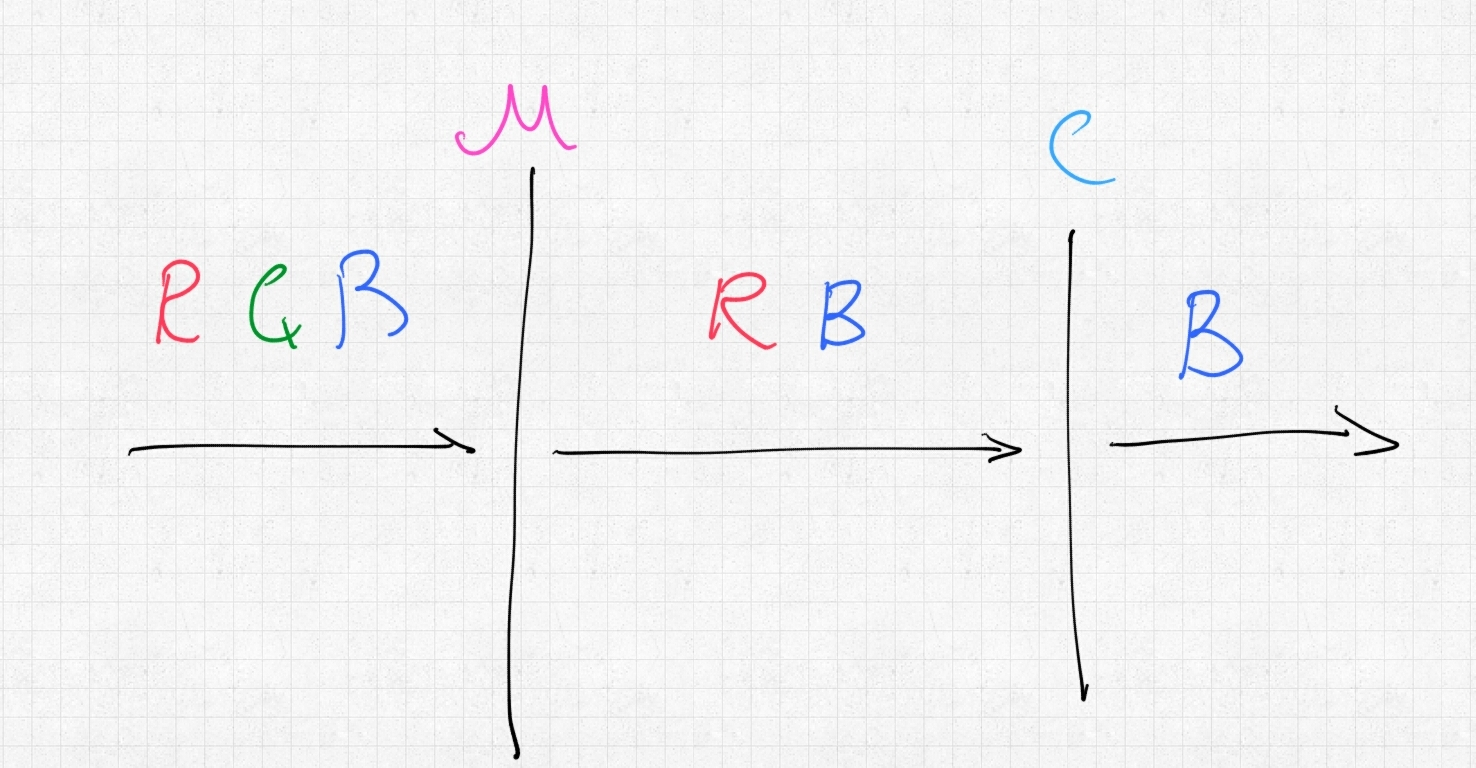
\includegraphics[width = 400px, keepaspectratio]{cmy}
\end{homeworkProblem}

\begin{homeworkProblem}
Suppose we have a 24 MP image (6000x4000). We would like to compare the
storage requirement for tuples (e.g., straight RGB storage) versus a single number
that is an index to a color tuple (e.g., how GIF represents images).
\begin{enumerate}[(a), leftmargin = 0.7cm, nosep]
\item Assuming 24-bit RGB values, how much memory would be required to represent
the image using straight tuples? \\

To represent 24MP image, using 24 bit RGB values we need $ 6000 \times 4000 \times 3 \times 24 =  576000000$ Bits \\
\pagebreak

\item Suppose we have a color table representation, where the index points to the color
value (remember, the color table needs to store the actual RGB values). What is the
total memory needed to represent the color table and represent the image, if the index
is 8-bits? 12-bits? 16-bits? and 20 bits? There is one answer for each. \\

Total memory for 8  bits = $ 256 * 8 * 24 =      49152     +  6000 * 4000 * 8  =      49152       +    192000000= 192049152 $  Bits \\
Total memory for 12 bits  = $ 4096 * 12 * 24 =    1179648   +  6000 * 4000 * 12 =      1179648     +    288000000= 289179648 $ Bits \\
Total memory for 16 bits  = $ 65536 * 16 * 24 =   25165824  +  6000 * 4000 * 16 =      25165824    +    384000000= 409165824 $ Bits \\
Total memory for 20 bits  = $ 1048576 * 20 * 24 = 503316480 +  6000 * 4000 * 20 =      503316480   +    480000000= 983316480 $ Bits \\


\item For the 8, 12, 16, and 20-bit indexes above, what is the maximum number of
colors that can be represented.\\

For 8  bits  = $ 2^8 = 256      $ Colors\\
For 12 bits  = $ 2^{12} = 4096   $ Colors\\
For 16 bits  = $ 2^{16} = 65536  $ Colors\\
For 20 bits  = $ 2^{20} = 1048576  $ Colors\\





\end{enumerate}
\end{homeworkProblem}

\end{document}
